\chapter{Implementazione dell'applicazione}
\pagestyle{plain}


\section{Introduzione}
In questa sezione andremo a descrivere l'implementazione andando a dare uno sguardo più profondo al codice e successivamente anche alle problematiche riscontrate surante lo sviluppo con le relative soluzioni.


\section{Gemini API}
\subsection{Structured output}

\begin{wrapfigure}[8]{r}{0.30\textwidth} %this figure will be at the right
    \centering
    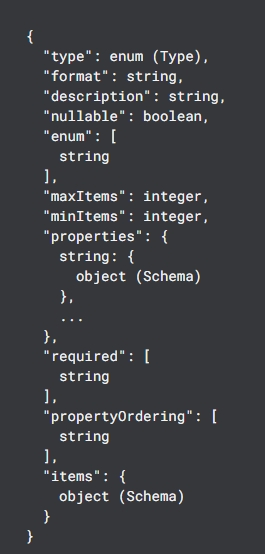
\includegraphics[width=0.30\textwidth]{figures/chapter_1/geminiPseudoSchema.png}
    \caption{Pseudo-JSON che rappresenta tutti i campi dello Schema}
\end{wrapfigure}

Lo Structured Output permette di farsi restituire da Gemini una risposta standardizzata, in questo caso un JSON, predefinita sotto forma di uno schema. Lo \textbf{Schema} supporta array, tipi e oggetti dentro i quali è possibile definire i tipi dei dati e i loro nomi. \cite{StructuredOutput}
I tipi nello \textbf{Schema} devono essere uno degli OpenAPI Data Types, oppure un'unione di questi tipi (utilizzando \texttt{anyOf}). Per ciascun tipo, è valido solo un determinato sottoinsieme di campi. Nella seguente lista viene riportata la corrispondenza tra ciascun tipo e il relativo insieme di campi validi:
\begin{itemize}
    \item \textbf{string}: \texttt{enum}, \texttt{format}, \texttt{nullable}
    \item \textbf{integer}: \texttt{format}, \texttt{minimum}, \texttt{maximum}, \texttt{enum}, \texttt{nullable}
    \item \textbf{number}: \texttt{format}, \texttt{minimum}, \texttt{maximum}, \texttt{enum}, \texttt{nullable}
    \item \textbf{boolean}: \texttt{nullable}
    \item \textbf{array}: \texttt{minItems}, \texttt{maxItems}, \texttt{items}, \texttt{nullable}
    \item \textbf{object}: \texttt{properties}, \texttt{required}, \texttt{propertyOrdering}, \texttt{nullable}
\end{itemize}

\begin{figure}[H]
    \centering
    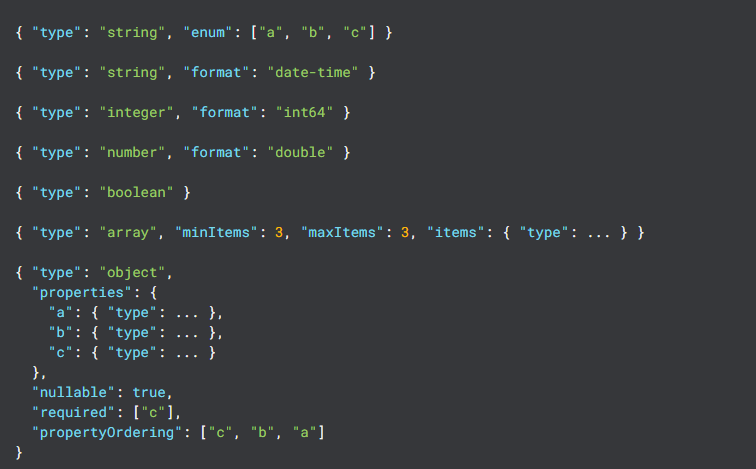
\includegraphics[width=0.8\textwidth,height=\textheight,keepaspectratio]{figures/chapter_1/GeminiSchema.png}
    \caption{Schemas di esempio}
\end{figure}

\subsection{Richieste POST}
Le richieste POST vengono fatte all'interno della classe \textbf{GeminiAPI}, che è anche la delegata al salvataggio dei dati ricevuti da Gemini in dei file JSON.

\begin{figure}[H]
    \centering
    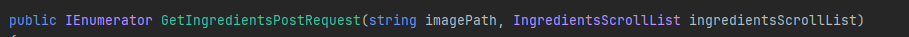
\includegraphics[width=0.8\textwidth,height=\textheight,keepaspectratio]{figures/chapter_1/GetIngredientsPostRequest.png}
    \caption{Funzione per generare gli ingredienti}
    \label{fig:getIngredientsPostRequest}
\end{figure}

\begin{figure}[H]
    \centering
    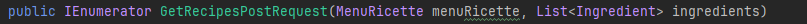
\includegraphics[width=0.8\textwidth,height=\textheight,keepaspectratio]{figures/chapter_1/GetRecipesPostRequest.png}
    \caption{Funzione per generare le ricette}
    \label{fig:getRecipesPostRequest}
\end{figure}

\subsubsection{Generazione degli ingredienti}
Per generare gli ingredienti useremo la funzione della fig.\ref{fig:getIngredientsPostRequest}. Il payload della  POST richiede: 
\begin{itemize}
    \item Una immagine in formato \texttt{Base64}
    \item L'API Key e l'API url di Gemini
    \item Lo schema che definisce i campi che Gemini deve restituire
\end{itemize}

Per convertire l'imagine in formato \texttt{Base64} useremo la funzione \texttt{Convert.ToBase64String()} di C\#. 
\begin{figure}[H]
    \centering
    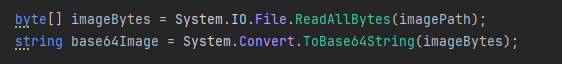
\includegraphics[width=0.8\textwidth,height=\textheight,keepaspectratio]{figures/chapter_1/base64.png}
    \caption{Lettura e conversione dell'immagine in Base64}
\end{figure}
\begin{figure}[H]
    \centering
    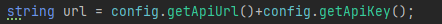
\includegraphics[width=0.8\textwidth,height=\textheight,keepaspectratio]{figures/chapter_1/APIkey.png}
    \caption{Creazione dell'url per la richiesta POST}
    \label{fig:apiKey}
\end{figure}
L'API Key e l'url vengono letti dal file config come in fig.\ref{fig:apiKey}, che poi vengono messi all'interno del payload, insieme allo schema mostrato in fig.\ref{fig:structuredOutput} e all'immagine in formato \texttt{Base64} mostrato in fig.\ref{fig:imagePayload}.

\begin{figure}[H]
    \centering
    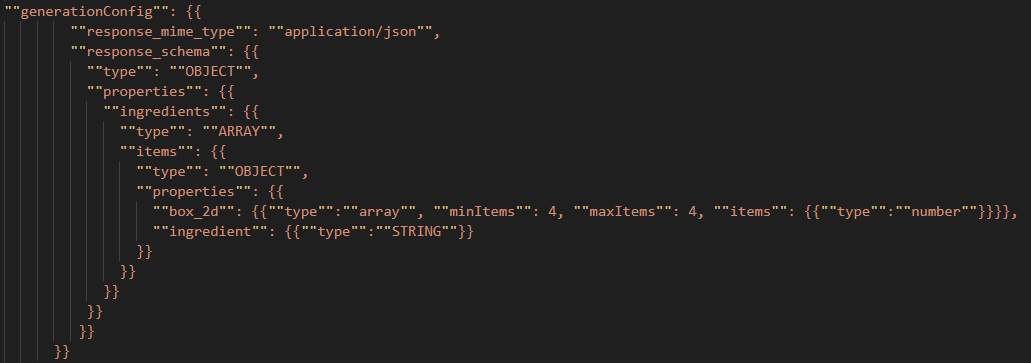
\includegraphics[width=0.8\textwidth,height=\textheight,keepaspectratio]{figures/chapter_1/StructuredOutput.png}
    \caption{Schema per la generazione degli ingredienti}
    \label{fig:structuredOutput}
\end{figure}
\begin{figure}[H]
    \centering
    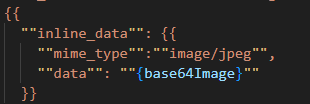
\includegraphics[width=0.5\textwidth,height=\textheight,keepaspectratio]{figures/chapter_1/imagePayload.png}
    \caption{Inserimento dell'immagine nel payload della richiesta POST}
    \label{fig:imagePayload}
\end{figure}
Infine viene effettuata la POST creando una nuova istanza della classe \textbf{UnityWebRequest}, convertendo il payload string in un array di byte per poi invocare il metodo \texttt{SendWebRequest()} per inviare la richiesta. Se la richiesta ha successo, Gemini risponderà con un JSON che contiene gli ingredienti, che verranno salvati in un file JSON.
\begin{figure}[H]
    \centering
    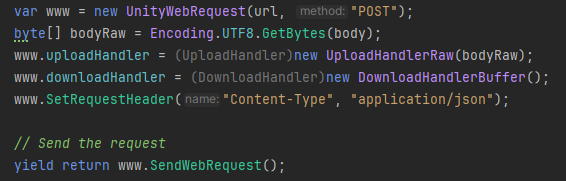
\includegraphics[width=0.6\textwidth,height=\textheight,keepaspectratio]{figures/chapter_1/richiestaPOST.png}
    \caption{Codice per effettuare la richiesta POST}
    \label{fig:postRequest}
\end{figure}

\subsubsection{Generazione delle ricette}
Per generare gli ingredienti useremo la funzione della fig.\ref{fig:getRecipesPostRequest}. In questo caso non ci servirà un'immagine ma la lista degli ingredienti, che verrà letta in un for e concatenata sotto un'unica stringa. La creazione dell'url e dell'API Key avviene come per la generazione degli ingredienti in fig.\ref{fig:apiKey}, ma lo Schema sarà diverso, come mostrato in fig.\ref{fig:recipeSchema}.

\begin{figure}[H]
    \centering
    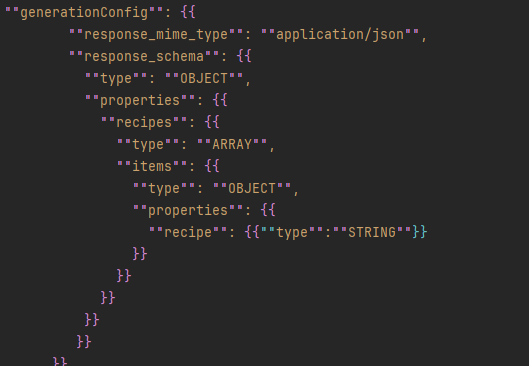
\includegraphics[width=0.6\textwidth,height=\textheight,keepaspectratio]{figures/chapter_1/recipeSchema.png}
    \caption{Schema per la generazione delle ricette}
    \label{fig:recipeSchema}
\end{figure}

Come possiamo facilmente notare lo schema è molto più semplice e richiede soltanto la restituzione di un array di oggetti, ognuno dei queli contiene una ricetta di tipo stringa.
Invece la richiesta testuale fatta è la seguente:
\begin{quote}
    \texttt{create three recipes only with the following ingredients: \{ingredientsConcat\}. Write it with tags compatible with TextMesh Pro, make the recipes titles colored in red, make the number of the instruction list colored in red, use bold in subtitles}
\end{quote}dove \texttt{ingredientsConcat} è la stringa che contiene tutti gli ingredienti separati da virgola.
L'invio della richiesta POST avviene come per la generazione degli ingredienti in fig.\ref{fig:postRequest}.

\section{File Handler}
la classe \textbf{FileHandler} è responsabile della lettura e scrittura e creazione dei file JSON. La particolarità è quella di essere una classe generica, in modo da poter serializzare tramite apposite classi serializzabili qualsiasi JSON.

\subsection{Classi Serializzabili}
Sono presenti quattro classi serializzabili, in particolare:
\begin{itemize}
    \item \textbf{ConfigJSON}: Serve a leggere il file di configurazione, dove sono salvati l'API Key, l'API URL di Gemini e i nomi dei file JSON da salvare e quello della foto.
    \item \textbf{GeminiResponseJSON}: Serve a leggere la risposta di Gemini che contiene gli ingredienti o le ricette e prendere i campi che ci interessano, in particolare il campo \texttt{text} tramite apposita funzione \texttt{GetText()}.
    \item \textbf{ListOfIngredientsJSON}: Utilizzata per salvare e leggere la lista degli ingredienti e ad assegnargli un ID univoco, che viene generato automaticamente quando si aggiunge un nuovo ingrediente.
    \item \textbf{ListOfRecipesJSON}: Utilizzata per salvare e leggere la lista delle ricette, che contiene un array di tipo \textbf{RecipesJSON}, ognuna delle quali contiene una stringa.
\end{itemize}

La separazione delle classi serializzabili da quelle del model permette di avere un codice più pulito e facilmente mantenibile, in quanto ogni classe ha una responsabilità ben definita.

\subsection{Metodi}
Sono presenti tre metodi:
\begin{itemize}
    \item \texttt{SaveJson(string jsonNameFile, T item)}: Salva un oggetto di tipo generico \textbf{T} nel file json con il nome passato tramite \textbf{jsonNameFile}. Il file viene creato se non esiste, altrimenti viene sovrascritto. Codice disponibile in fig.\ref{fig:saveJson}.
    \item \texttt{public T LoadJson(string jsonNameFile)}: deserializza un file JSON con il nome passato tramite \textbf{jsonNameFile} e restituisce un oggetto di tipo generico \textbf{T}. Se il file non esiste, ne viene creato uno vuoto e viene restituito un oggetto di tipo generico \textbf{T} vuoto. Codice disponibile in fig.\ref{fig:loadJson}.
    \item \texttt{CreateBlankFile(string filePath)}: Crea un file vuoto con il nome passato tramite \textbf{filePath}. Se il file esiste già, non viene creato nulla.
\end{itemize}

\begin{figure}[H]
    \centering
    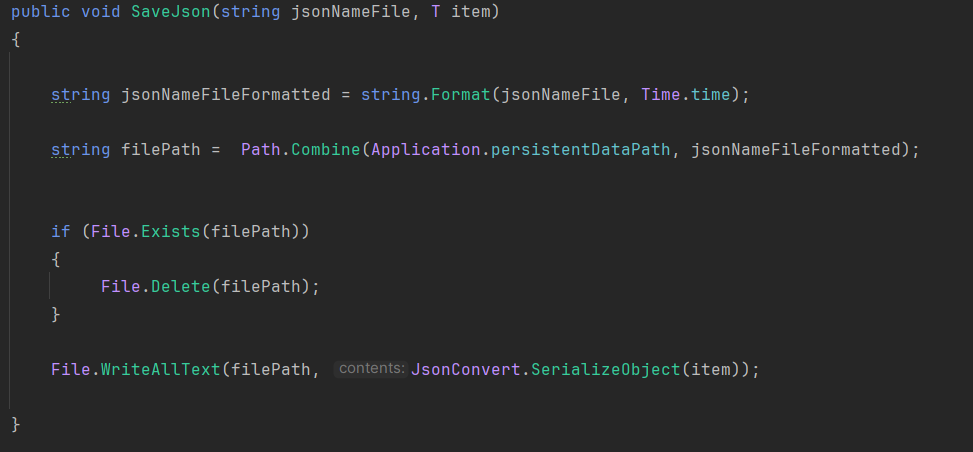
\includegraphics[width=0.6\textwidth,height=\textheight,keepaspectratio]{figures/chapter_1/saveJson_CODICE.png}
    \caption{Codice per effettuare il salvataggio del JSON}
    \label{fig:saveJson}
\end{figure}
\begin{figure}[H]
    \centering
    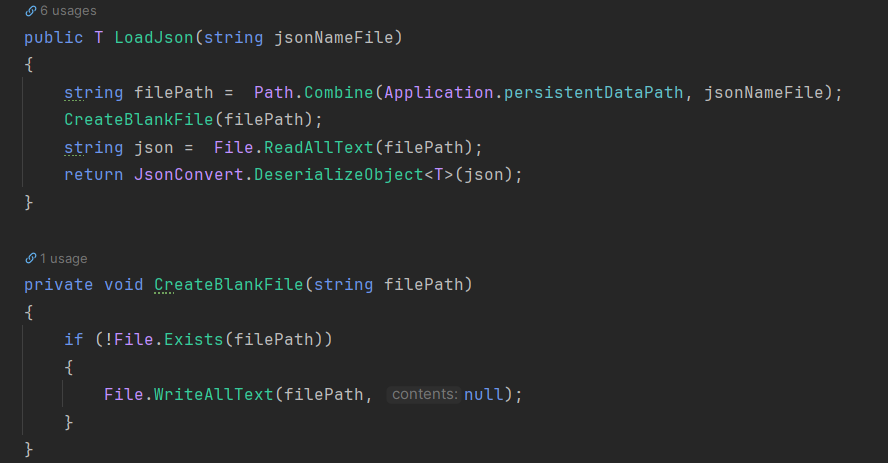
\includegraphics[width=0.6\textwidth,height=\textheight,keepaspectratio]{figures/chapter_1/LoadJson_CODICE.png}
    \caption{Codice per effettuare la deserializzazione del JSON}
    \label{fig:loadJson}
\end{figure}

\section{Scatto della foto}
Per scattare la foto usiamo la classe \textbf{PhotoShooter}, che utilizza la libreria \\ \textbf{UnityEngine.Windows.WebCam} di Unity per accedere alla fotocamera del dispositivo. La classe è responsabile della gestione della fotocamera, dello scatto della foto e del salvataggio dell'immagine in un file ed è implemantata tramite un singleton per garantire che ci sia una sola istanza della classe durante l'esecuzione dell'applicazione.
Sono presenti due funzioni principali:
\begin{itemize}
    \item \texttt{TakePhoto(string photoPath)}: controlla se la foto non esiste già, altrimenti la cancella e crea un processo asincrono per scattare e salvare la foto. Fig.\ref{fig:takePhoto}
    \item \texttt{DeletePhoto(string photoPath)}: cancella la foto scattata, se esiste. Fig.\ref{fig:deletePhoto}
\end{itemize}

\begin{figure}[H]
    \centering
    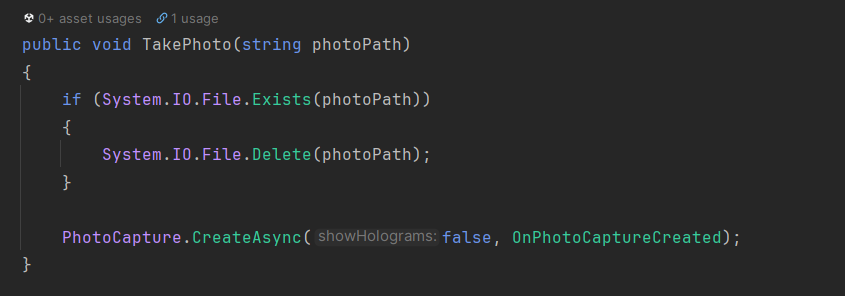
\includegraphics[width=0.6\textwidth,height=\textheight,keepaspectratio]{figures/chapter_1/TakePhoto_CODICE.png}
    \caption{Inizio funzione per lo scatto della foto}
    \label{fig:takePhoto}
\end{figure}
\begin{figure}[H]
    \centering
    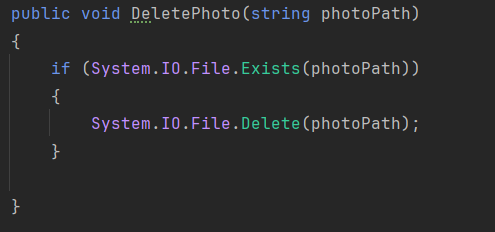
\includegraphics[width=0.6\textwidth,height=\textheight,keepaspectratio]{figures/chapter_1/DeletePhoto_CODICE.png}
    \caption{Codice per l'eliminazione della foto}
    \label{fig:deletePhoto}
\end{figure}
\begin{figure}[H]
    \centering
    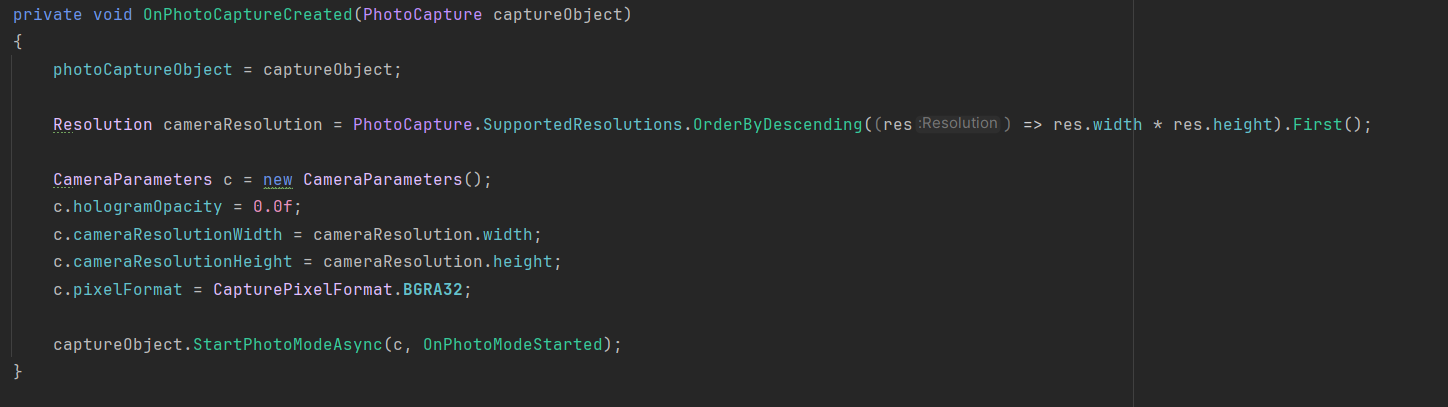
\includegraphics[width=1\textwidth,height=\textheight,keepaspectratio]{figures/chapter_1/OnPhotoCaptureCreated_CODICE.png}
    \caption{Inizializzazione della fotocamera}
    \label{fig:onPhotoCaptureCreated}
\end{figure}
Nella figura \ref{fig:onPhotoCaptureCreated} il metodo \textbf{OnPhotoCaptureCreated} viene inizializzata la fotocamera con la massima risoluzione possibile e iniziata la cattura della foto in maniera asincrona utilizzando il metodo \textbf{OnPhotoModeStarted}

\begin{figure}[H]
    \centering
    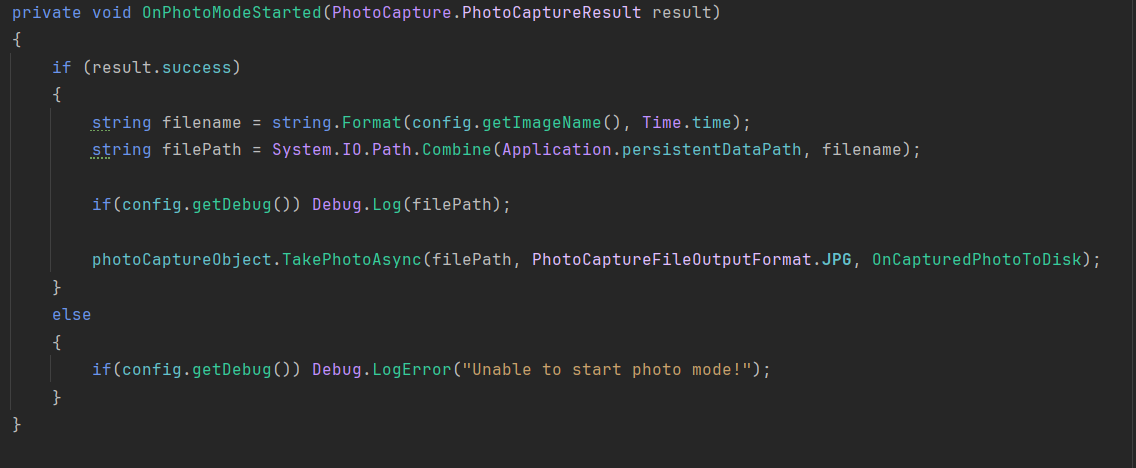
\includegraphics[width=0.9\textwidth,height=\textheight,keepaspectratio]{figures/chapter_1/OnPhotoModeStarted_CODICE.png}
    \caption{Scatto della foto}
    \label{fig:onPhotoModeStarted}
\end{figure}
Nella figura \ref{fig:onPhotoModeStarted} il metodo \textbf{OnPhotoModeStarted} viene chiamato in maniera asincrona e tramite
\begin{lstlisting}[language=java]
    photoCaptureObject.TakePhotoAsync(filePath, PhotoCaptureFileOutputFormat.JPG, OnCapturedPhotoToDisk); 
\end{lstlisting}
    viene scattata la foto e utilizzato il metodo \textbf{OnCapturedPhotoToDisk} per salvare la foto su disco al path precedentemente definito dal \textbf{persistentDataPath}.

\begin{figure}[H]
    \centering
    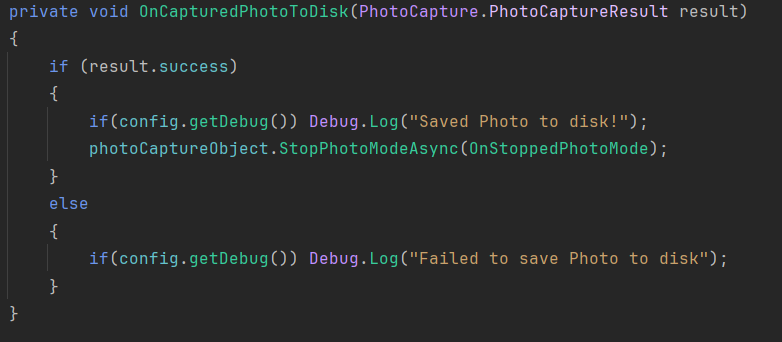
\includegraphics[width=0.6\textwidth,height=\textheight,keepaspectratio]{figures/chapter_1/OnCapturedPhotoToDisk_CODICE.png}
    \caption{Salvataggio della foto su disco}
    \label{fig:onCapturedPhotoToDisk}
\end{figure}

In figura \ref{fig:onCapturedPhotoToDisk} il metodo \textbf{OnCapturedPhotoToDisk} è utilizzato per salvare la foto su disco, se l'operazione è compiuta con successo viene chiamato il metodo \textbf{OnStoppedPhotoMode} per terminare la modalità foto e rilasciare le risorse della fotocamera.


\begin{figure}[H]
    \centering
    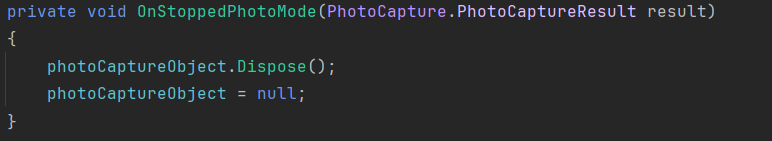
\includegraphics[width=0.6\textwidth,height=\textheight,keepaspectratio]{figures/chapter_1/OnStoppedPhotoMode_CODICE.png}
    \caption{Procedura per terminare lo scatto della foto}
    \label{fig:onStoppedPhotoMode}
\end{figure}

In figura \ref{fig:onStoppedPhotoMode} il metodo \textbf{OnStoppedPhotoMode} viene chiamato per terminare la modalità foto e rilasciare le risorse della fotocamera, in particolare tramite \texttt{photoCaptureObject.Dispose()} il cui metodo \texttt{Dispose()} viene chiamato per arrestare l'istanza di \textbf{PhotoCapture}.

\section{Lista ingredienti}
Possiamo definire la lista degli ingredienti come uon dei più complessi elementi presenti nell'applicazione, in quanto è composta da dei prefab che vengono visualizzati in una lista, ognuno dei quali contiene il nome dell'ingrediente modificabile e eliminabile.
\subsection{Prefab}
Utilizzando il prefab \textbf{IngredientButtonRow} possiamo visualizzare gli ingredienti all'interno della lista, riusciendolo a generarlo quanti sono gli ingredianeti presenti nel file JSON.
\begin{figure}[H]
    \centering
    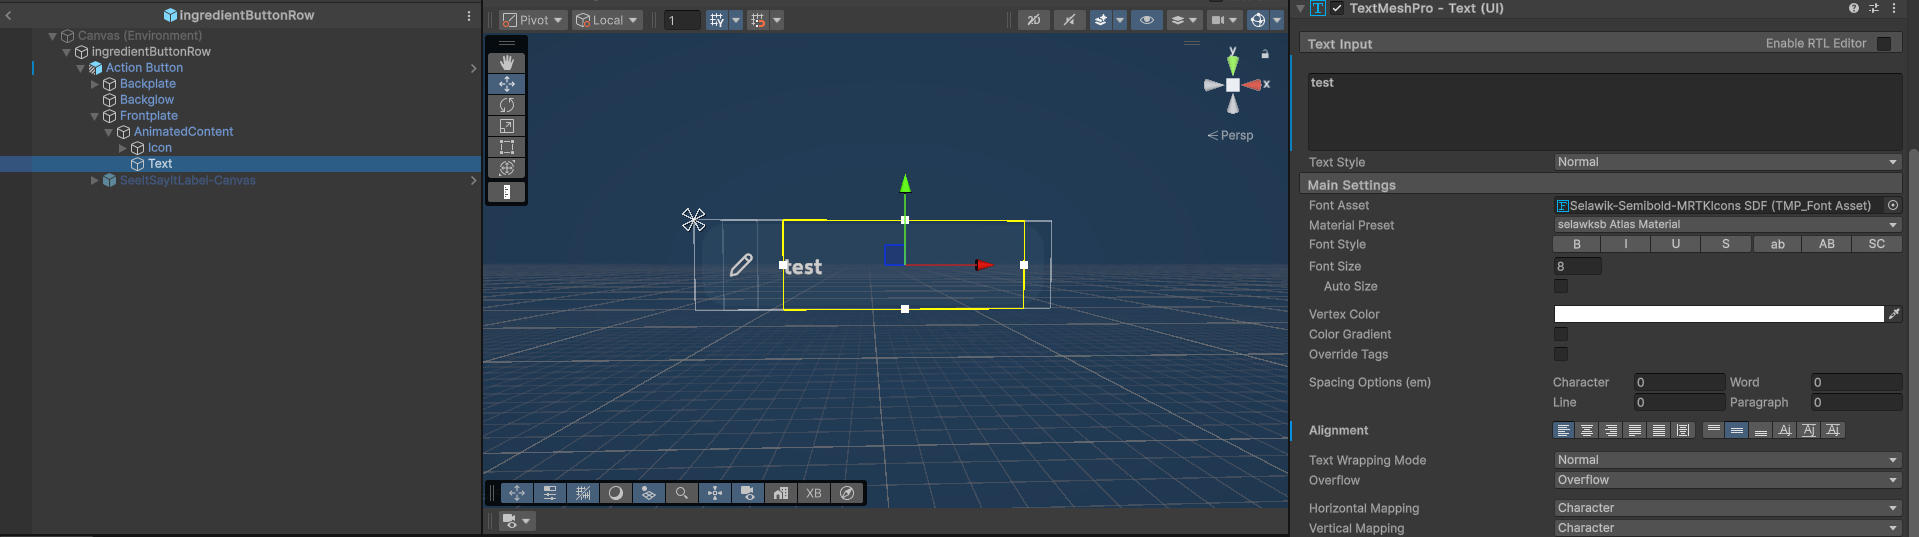
\includegraphics[width=1\textwidth,height=\textheight,keepaspectratio]{figures/chapter_1/prefab.png}
    \caption{Gerarchia del prefab IngredientButtonRow}
    \label{fig:prefab3D}
\end{figure}
Il prefab è un bottone al cui interno è presente un \textbf{TextMeshPro} per il nome dell'ingrediente, se cliccato verrà aperta la schermata di modifica del'ingrediente. 
Al prefab è assegnato uno script \textbf{IngredientButtonRow} che contiene i metodi per l'inizializzazione del prefab e il funzionamento generale.
\begin{figure}[H]
    \centering
    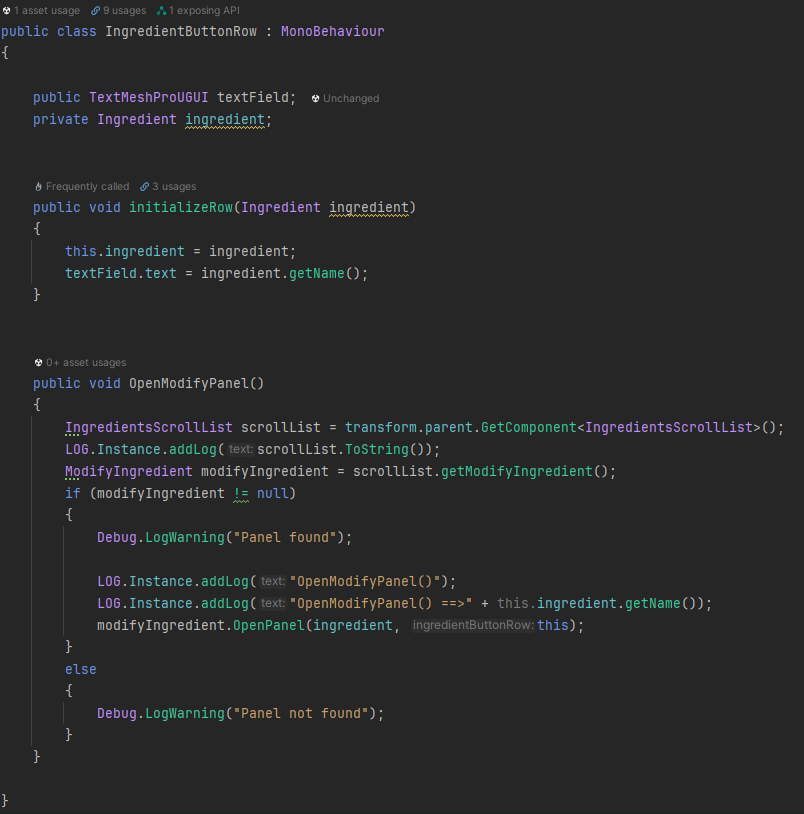
\includegraphics[width=0.9\textwidth,height=\textheight,keepaspectratio]{figures/chapter_1/prefab_CODICE.png}
    \caption{Classe IngredientButtonRow}
    \label{fig:prefabCodice}
\end{figure}

La variabile \textbf{TextField} è di tipo \textbf{TextMeshProUGUI} e rappresenta il campo di testo del nome dell'ingrediente, componente del prefab, e visto che è serializzabile e dichiarata come pubblica questa verrà mostrata nell'Inspector di Unity, permettendo di assegnare il campo di testo direttamente dal prefab con un drag and drop.\\
Il metodo \texttt{InitializeRow(Ingredient ingredient)} viene chiamato per inizializzare il prefab con i dati dell'ingrediente passato come parametro, in particolare viene assegnato il nome dell'ingrediente al campo di testo \textbf{TextField} e salvato nella variabile \textbf{ingredient}.
\subsection{Creazione del prefab all'interno della lista}
La scroll list, come visto in fig.\ref{fig:scrollablePanel}, è formata da diversi oggetti nella gerarchia, tra cui il \textbf{Content}, ossia l'ultimo elemento della gerarchia ma il padre dei prefab generati. Infatti proprio questo oggetto è delegato alla loro creazione, modifica e cancellazione.
\begin{figure}[H]
    \centering
    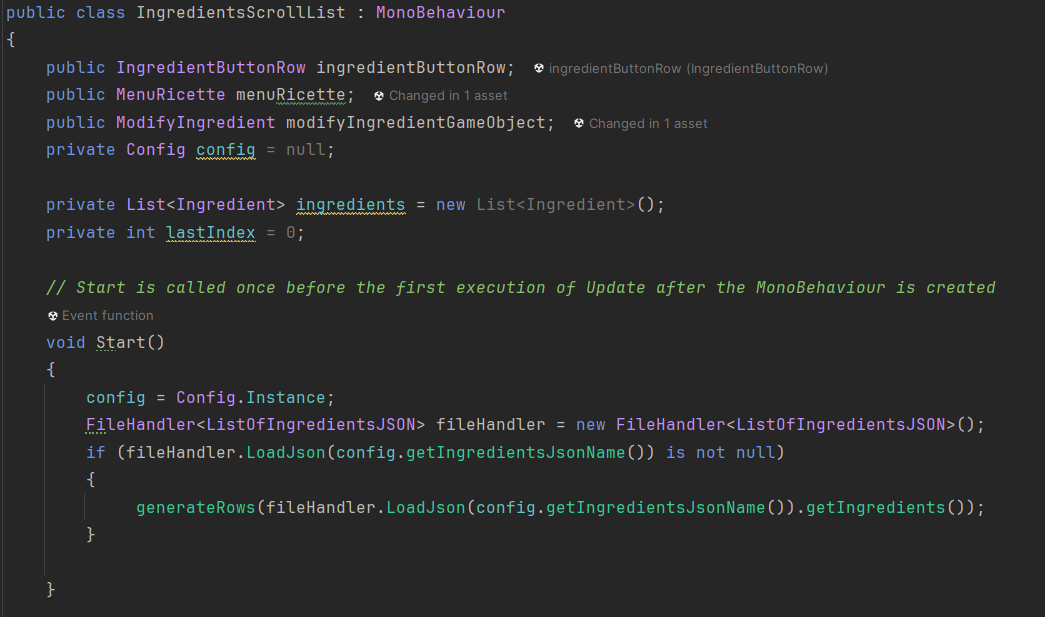
\includegraphics[width=0.9\textwidth,height=\textheight,keepaspectratio]{figures/chapter_1/IngredientsScrollList_START.png}
    \caption{Dichiarazione delle variabili e metodo Start}
    \label{fig:ingredientsScrollListStart}
\end{figure}

Fra le diverse variabli dichiarate troviamo \textbf{ingredients}, una lista di tipo \textbf{Ingredient} che andremo a popolare alla chiamata del metodo Start. \\
Nel metodo \texttt{Start()} tramite la classe \textbf{FileHandler} andremo a leggere il file JSON degli ingredienti, se il metodo \texttt{LoadJson()} non è nulla allora chiamiamo la funzione \texttt{getIngredients()} implementata nella classe per serializzare il JSON, che resituisce una lista di ingredienti. Questa lista viene passata al metodo \texttt{generateRows()} che si occupa di  generare i prefab per ogni ingrediente presente nella lista \textbf{ingredients} e di aggiornare la variabile \textbf{ingredients} per poi generare i prefab all'interno della lista.
\begin{figure}[H]
    \centering
    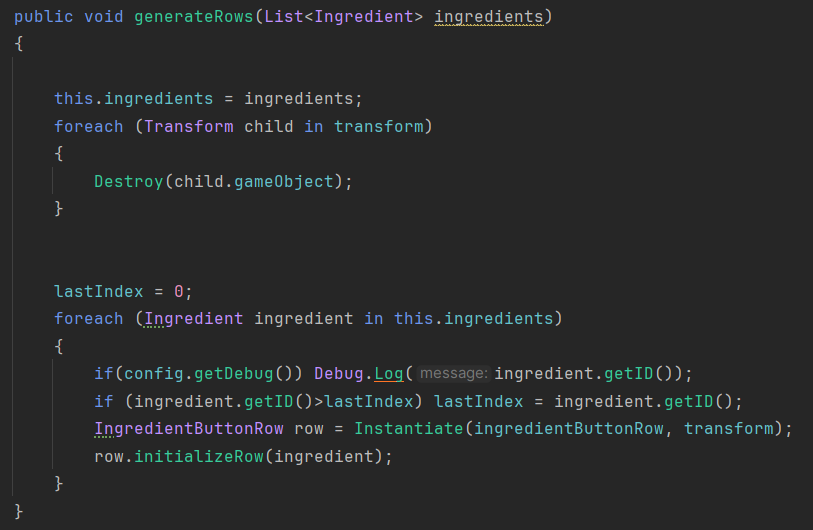
\includegraphics[width=0.9\textwidth,height=\textheight,keepaspectratio]{figures/chapter_1/generateRows_CODICE.png}
    \caption{Metodo per generare i prefab}
    \label{fig:generateRows}
\end{figure}
Il metodo \texttt{generateRows()} si occupa di generare i prefab per ogni ingrediente presente nella lista \textbf{ingredients}. Prima di tutto aggiorna la variabile \textbf{ingredients} con la lista degli ingredienti passata come parametro, poi se al suo interno ha dei figli vengono distrutti tramite un ciclo \texttt{foreach}, successivamente, sempre con un ciclo \texttt{foreach} per ogni ingrediente presente nella lista \textbf{ingredients} viene generato un prefab. La creazione del prefab viene spiegata al paragrafo \ref{sec:prefab}, aggiungiamo solo che il prefab viene generato tramite il metodo \texttt{Instantiate()} di Unity, che prende come parametro il prefab da generare e la posizione in cui generarlo, in questo caso la posizione è quella del \textbf{Content} della lista, per questo per semplicità è stato passato direttamente \textbf{transform}. Il prefab viene poi assegnato alla variabile \textbf{ingredientButtonRow} e viene chiamato il metodo \texttt{initializeRow()} passandogli come parametro l'oggetto di tipo \textbf{Ingredient}.

\subsection{Aggiunta, modifica e cancellazione}
Le funzionalità di aggiunta, modifica e cancellazione degli ingredienti sono delegate sempre alla classe \textbf{IngredientsScrollList}, tramite gli appositi metodi \texttt{addIngredient(string ingredientName)}, \texttt{ deleteIngredient(Ingredient ingredient, IngredientButtonRow ingredientButtonRow)} e \\ \texttt{modifyIngredient(Ingredient oldIngredient, Ingredient newIngredient, \\ IngredientButtonRow ingredientButtonRow)}. Inoltre è presente un metodo \texttt{saveList()} che si occupa di salvare la lista degli ingredienti nel file JSON, chiamato alla fine di ogni operazione di modifica della lista.

\begin{figure}[H]
    \centering
    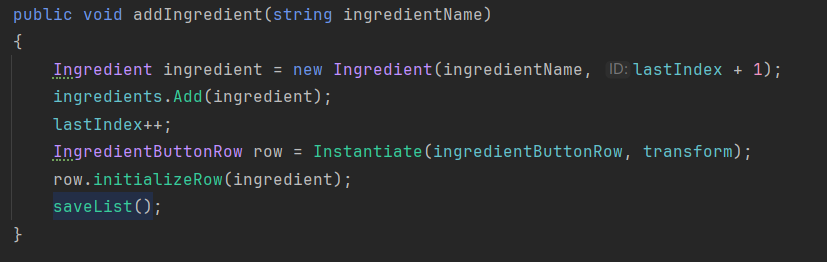
\includegraphics[width=0.9\textwidth,height=\textheight,keepaspectratio]{figures/chapter_1/addIngredient_CODICE.png}
    \caption{Metodo per aggiungere un ingrediente}
    \label{fig:addIngredient}
\end{figure}
\begin{figure}[H]
    \centering
    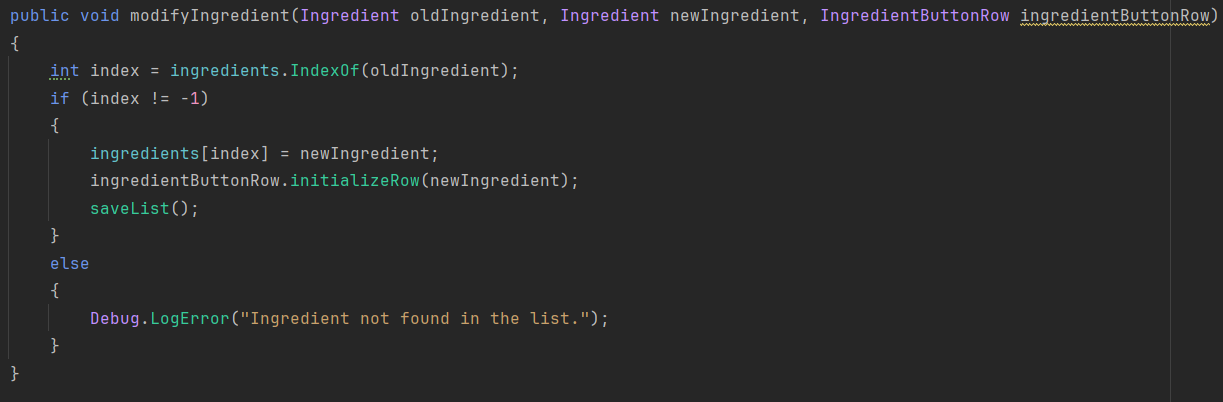
\includegraphics[width=1\textwidth,height=\textheight,keepaspectratio]{figures/chapter_1/modifyIngredient_CODICE.png}
    \caption{Metodo per modificare un ingrediente}
    \label{fig:modifyIngredient}
\end{figure}
\begin{figure}[H]
    \centering
    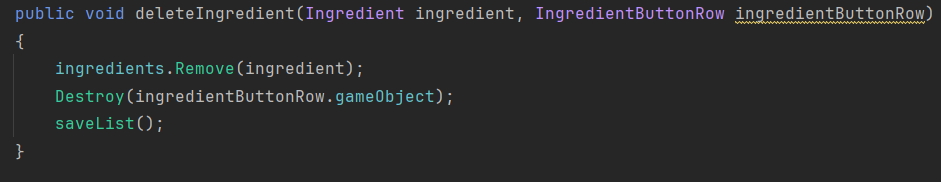
\includegraphics[width=0.9\textwidth,height=\textheight,keepaspectratio]{figures/chapter_1/deleteIngredient_CODICE.png}
    \caption{Metodo per cancellare un ingrediente}
    \label{fig:deleteIngredient}
\end{figure}
\begin{figure}[H]
    \centering
    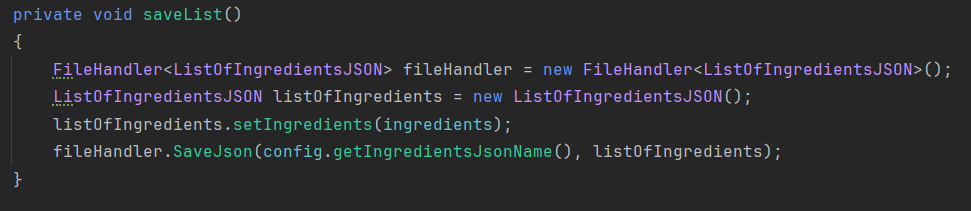
\includegraphics[width=0.9\textwidth,height=\textheight,keepaspectratio]{figures/chapter_1/saveList_LISTA_CODICE.png}
    \caption{Metodo per salvare la lista degli ingredienti}
    \label{fig:saveListScrollList}
\end{figure}



\section{Tastiera virtuale}
\section{Problematiche e soluzioni} 
